\chapter{Az alkalmazás felépítése}

Először az alkalmazás felépítését csak nagyvonalakban, funkcionális egységenként kell részletezni. Kvázi a tipikus kliens-szerver-es architektúrát kell személyre szabni kicsit.

Ebbe a részbe következik majd aztán a felhasznált technológiák bemutatása. Itt annak kell érződnie, hogy minden eszköz a problémának megfelelően lett megválasztva.

Már itt célszerű azt is láthatóvá tenni, hogy hol érnek véget a library-k és keretrendszerek, és mi az ami saját készítésű. Nem tudni, hogy milyen szinten lesz otthon ezekben az, aki olvassa, ezért jól láthatóvá kell tenni, hogy melyik komponens/kódrész mit csinál, és hogy saját készítésű, vagy készen felhasznált.

\section{Felhasznált eszközök és technológiák}

A feladatom webalkalmazás készítése éttermek és rendelések adatainak nyilvántartásához. Ennek megvalósításához a Python programozási nyelvet, és a flask webes keretrendszert választottam.

Felhasználói felület létrehozása webes környezetben HTML5 és AngularJS segítségével történt.

Az adatokat SQLite alapú relációs adatbázisban tárolom, amelyhez a keretrendszer SQLAlchemy ORM-en keresztül csatlakozik. 

A dolgozatom készítése során a GitHub nevű online verziókövető rendszert használtam.

\subsection{Git}

A Git jelenleg a világon a legszélesebb körben használt modern verziókezelő rendszer. A Git egy nyílt forráskódú, elosztott verzió követő rendszer, melyet 2005-ben fejlesztett ki LinusTorvalds, a Linux kernel atyja. Minden Git munkamásolat egy teljes értékű repository teljes verziótörténettel és teljes revíziókövetési lehetőséggel, amely nem függ a hálózat elérésétől vagy központi szervertől. Számos nagy volumenű projekt használja jelenleg a Gitet verziókezelő rendszerként.

\subsection{GitHub}

A GitHub egy Git alapú verziókövető tárhely, és egyben egy ingyenes internetes tárhely. Szolgáltatja az elosztott verziókezelő rendszer, és a forrás kód menedzselés minden funkcióját. Biztosítja a hozzáférés-szabályozást és még számos más funkciót, mind például a bug tracking, feature requests, vagy task managment.

Ezek tudatában választottam a GitHubot verziókezelő rendszernek.

\subsection{Python}

A Pythont Guido van Rossum holland programozó kezdte el fejleszteni 1989 végén. A Python egy ––széles körben használt, nagyon magas szintű általános célú programozási nyelv. Ez egy úgynevezett interpreteres nyelv, ami azt jelenti, hogy nincs különválasztva a tárgykód és a forráskód. A Python iterpretert számos géptípusra és operációs rendszerre elkészítették. A nyelvnek van egy sajátos tervezési filozófiája, ami az olvashatóságot, és a programozói munka megkönnyítését helyezi előtérbe, olyan szintaxisa van, amely lehetővé teszi a programozók számára, hogy kevesebb kódsoron fogalmazzák meg a koncepciókat, mint például a C\# vagy a Java nyelvek esetében.

A Python támogatja a dinamikus típusokat és az automatikus memória kezelést, emellett szigorú típusrendszerrel rendelkezik. Számos programozási paradigmát támogat, mint például az objektumorientált, funkcionális, imperatív vagy procedurális.

\subsection{Flask}

Miután kiválasztottam a Python-t, szükségem volt még az alkalmazásom elkészítéséhez egy webes keretrendszerre. Számos python alapú webes keretrendszert találtam, ezek közül hárommal szimpatizáltam. Ez a három a Django, a Flask és a Pyramid volt. Miután összevettem őket, arra a következtetésre jutottam, hogy a feladatom megvalósításához a Flask lesz a legalkalmasabb.
A Flask lényegében egy Python nyelven íródott Werkzeug eszközrendszeren alapuló, Jinja2 template motort használó webes mikro - keretrendszer. A Flaskot azért nevezik mikro- keretrendszernek, mert nem igényel speciális eszközöket vagy könyvtárakat. Nem rendelkezik adatbázis-absztrakciós réteggel, form validációval, vagy bármely más olyan összetevővel, ahol már létező, harmadik féltől származó könyvtárak közös funkciókat biztosítanak. Azonban, a Flask olyan bővítményeket támogat, melyek képesek alkalmazási funkciók hozzáadására, úgy mintha azok eleve implementálva lettek volna a flaskban. Bővítmények léteznek az objektum-relációs mapperekre, form validációra, feltöltés kezelésére és még számos közös keretrendszerhez kapcsolódó eszközre. Ezeknek a bővítményeknek sokkal gyakrabban jön ki friss verziójuk, mint magának a Flasknak.

\subsection{Pycharm}

A Pycharm a JetBrains által fejlesztett Python integrált fejlesztői környezet. A Pycharm biztosít kód analízist, grafikus debuggert, egy integrált egység tesztelőt, integrációt verzió kezelő rendszerrel, és támogatja a web fejlesztést.
Azért esett erre a fejlesztői környezetre a választásásom, mert korábban már használtam a JetBrains által fejlesztett szoftvereket, és nagyon elégedett voltam velük. Megbízható, stabil, gyors, és nagyon sok alap funkció van bele integrálva, tehát nem kell különféle pluginokat telepítenem, mint például az Eclipse esetében.

\subsection{HTML5}

A HTML (angolul HyperText Markup Language) egy általános leíró nyelv, melyet weboldalak és webes alkalmazások készítésre használnak. A HTML mára már internetes szabvánnyá vált a W3C (World Wide Web Consortium) támogatásával.
A HTML5 az ötödik és egyben a jelenleg a legjelentősebb verziója a HTML-nek. 2014 októberében publikálta a W3C, a fejlesztés egyik fő célja, hogy a webes alkalmazásokhoz ne kelljen telepíteni a különböző multimédiás plugineket. A HTML5 visszamenőleges kompatibilitást biztosít.
Cascading Style Sheets (CSS)

A stíluslapok úgynevezett stílusszabályokból állnak, melyeket egy stílusleíró nyelven adunk meg, ez a stílusleíró nyelv a Többszintű Stíluslapok nyelve, azaz a CSS. A CSS segítségével tudjuk leírni a jelölőnyelv alapú (például HTML) strukturált dokumentumok megjelenését. Megadhatjuk az HTML dokumentum minden egyes elemének a stílusát. A stíluslap minden eleme kijelölőből (selector) és meghatározásból (declaration) áll.

\subsection{Bootstrap}

A Bootstrap egy ingyenes, nyílt forráskódú front-end webes keretrendszer weboldalak és webes alkalmazások megjelenésének tervezésére. HTML és CSS alapú sablonokat tartalmaz a betűtípusok, formok, gombok, egyéb interfész-összetevők, valamint az opcionális JavaScript bővítmények számára. A Bootstrap ellentétben más webes keretrendszerekkel, csak front-end fejlesztéssel foglalkozik. A Bootstrap az egyik legnépszerűbb keretrendszer, melyet responsive webes alkalmazások fejlesztésére használnak.
JavaScript

A JavaScript egy Netscape által fejlesztett, interpreteres programozási nyelv. Gyengén típusos, dinamikus nyelv, amely lehetővé teszi dinamikus események kiváltását HTML alapú weboldalakon. Javan alapul, közvetlenül HTML dokumentumba épül be és a webböngésző értelmezi.

\subsection{AngularJS}

Az AngularJS egy JavaScript alapú nyílt forráskódú front-end webes keretrendszer, melyet főként single-page alkalmazások fejlesztésénél használnak. Az AngularJS felfogható egy MVC keretrendszernek. Model réteg alatt a JavaScript változókat kell érteni, melyek az adatokat tárolják. A view réteg maga a HTML kód, amit az AngularJS további beágyazott egyedi tag attribútumokkal egészít ki. Ezek a beágyazott attribútumok rendelik össze a view réteget a model és controller rétegekkel. A controller réteget a Javascript függvények adják, amik módosítják a model rétegben lévő JS változókat.
A JavaScript analitikai szolgáltatása a Libscore szerint az AngularJS-t használja a Wolfram Alpha, NBC, Walgreens, Intel, Sprint, ABC News, valamint a 2016 októberében tesztelt 1 millió weblap közül további 12000. Az AngularJS jelenleg benne van a top 100 legelterjedtebb GitHub projekt között.

\subsection{SQLAlchemy}

Az SQLAlchemy a Pythonhoz írt nyílt forráskódú ORM rendszer Széles körű szolgáltatást nyújt adatbázis függetlenül, kezdve az egyszerű lekérdezés generálástól az átfogó, akár többszörös összekapcsoláson át egészen a táblák alapvető információinak kinyeréséig. Könnyű használhatósága és teljesítménye miatt ez a ma leggyakrabban használt ORM eszköz Python rendszerekhez. 
Az SQLAlchemy egyik nagy előnye, hogy képes egyszerre magas és alacsony szintű absztrakciót nyújtani, a rendszer elvárásától függően. A leggyakrabban használt python keretrendszerek, mint például a Flask vagy a Django, nagy mértékű támogatást nyújtanak hozzá, ennek köszönhetően nagyon fejlesztőbarát megoldásnak tekinthető.

\section{Funkcionális specifikáció}

- Word-ös változatból át lehet ide rakni a dolgokat.
- Use-case diagram nem feltétlen kell.

\section{A szoftver architektúrája}

Komponens diagram, blokk diagram

Például:
- statisztikai elemző rész
- jogosultságok kezelése
- tárolás, biztonsági mentés
- körlevelek kezelése (például akciókhoz, új termékekhez)
- levelezőrendszer
- webszerver
- adatbázisszerver
- ajánlórendszer

Rendszer indítási folyamata

Protokollok az egyes elemek között

\section{Az alkalmazás fő részei}

Az alkalmazás szerveroldalon a \textit{Python/Flask} keretrendszert, kliensoldalon pedig \textit{AngularJS}-t használ. Az adatokat relációs adatbázisban tárolom, amelyhez a keretrendszer \textit{SQLAlchemy ORM}-en keresztül csatlakozik. Létrehoztam egy nyilvántartás nevű csomagot, ami alacsonyabb szintű programészre épülve magasabb szintű funkciókat valósít meg, elfedve a technikai részleteket. Az alkalmazás logikai felépítést \aref{fig:architecture}. ábra szemlélteti.

\begin{figure}
\centering
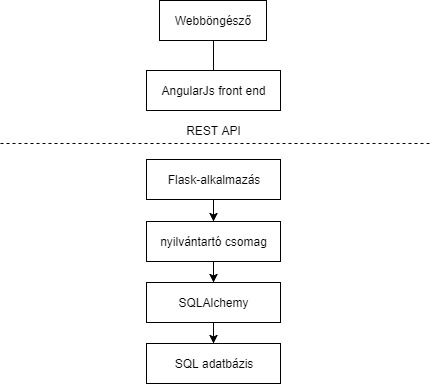
\includegraphics[scale=0.8]{kepek/architecture.jpg}
\caption{A webalkalmazás architektúrája}
\label{fig:architecture}
\end{figure}

A felhasználó böngészőn keresztül tudja használni az alkalmazást. Az alkalmazás használója ilyenkor az AngularJs-sel kialakított úgy nevezett nézeteket látja. Kliens oldalon az Angular kontrollerjei végzik a kérések elküldését a szerver irányába, melyekre a szerver az adatok visszaküldésével válaszol. A kapott válaszokat szintén az kontrollerek dolgozzák fel. A felhasználói felületről és az Angularról az ötödik fejezetben fogok bővebben írni.

% TODO: Apróság, de a fejezetet itt is majd \ref-el kellene hivatkozni!

A szerver oldalon egy többrétegű struktúrát hoztam létre. Az alsó réteg az adatbázis, ami egy SQLite alapú relációs adatbázis, amelyhez a keretrendszer SQLAlchemy ORM-en keresztül csatlakozik, tehát a lekérdezéseket az SQLAlchemy-vel végzem. Az SQL adatbázist a 4. fejezetben fogom részletesebben taglalni.

A klienstől érkező kérések feldolgozására az alkalmazás a Flask webes mikro keretrendszert használja. A flaskos réteg http válaszokat küld a kliensnek, melyeben az adatok JSON formátumúak. A flaskos réteg és az alsóbb rétegek között van egy közbenső réteg, az általam készített nyilvántartó csomag. A nyilvántartó csomagban lévő metódusok végzik a lekérdezéseket, ezeket a metódusokat hívom meg a flaskos rétegben. A közbenső réteg bevezetésére a későbbi továbbfejlesztési lehetőségek miatt volt szükség. A flask és a nyilvántartó csomag bemutatására a hetedik fejezben fog sor kerülni.

\section{Az alkalmazás alapfunkciói}

Az alkalmazásom lényegében éttermek és rendelések adatainak nyilvántartására fog szolgálni. Ebben a fejezetben az alap funkcionalitásokat fogom tárgyalni.

\section{Bejelentkezés/ regisztráció}

Az alkalmazásom egyik alap funkcionalitása a felhasználókezelés lesz. Csak regisztrált felhasználók számára lesznek elérhetőek a szolgáltatások, a kezdőlapon lesz lehetőség a bejelentkezésre, vagy regisztrációra. Alapvetően két felhasználói csoportot lehet majd megkülönböztetni, a vásárlókat és az étterem tulajdonosokat. A két csoport eltérő jogosultsági körrel fog rendelkezni, és más-más szolgáltatások lesznek számukra elérhetőek.

\section{Vásárlók funkciói}

\subsection{Böngészés az éttermek között}

A vásárlóknak lehetőségük lesz az adatbázisban szereplő éttermek kínálatai között böngészni. Szűrési feltételek megadásával szűkíthetik a kilistázott éttermek listáját, hogy megtalálják a számukra legszimpatikusabbat.
A kívánt étterem kiválasztása után a server kilistázza az adott étterem által kínált termékeket. A termékek között is lesz lehetőség szűrésre például típus szerint. A megrendelendő termékeket a vásárló belehelyezheti a kosárba. A kosár tartalma egy angular változóban lesz letárolva. A kosár tartalma is módosítható lesz.

\subsection{Rendelés}

A rendelés véglegesítése előtt a vásárlónak lehetősége lesz kiválasztani a kívánt fizetési módot. Rendelés során a kosár tartalma elküldésre kerül a servernek. A server létrehozza a szükséges order és \texttt{order\_meals} objektumokat, majd letárolja őket az adatbázisban. A rendelésről visszajelzést fog kapni a vásárló és az étterem tulajdonosa is. A rendelések adatait később statisztikák, kimutatások készítésénél lehet majd felhasználni.

\subsection{Felhasználói adatok}

A felhasználók számára lesz egy szolgáltatás, amely kilistázza az adott account adatait.

\subsection{Jelszó módosítás}

A felhasználói adatok kilistázása mellett lehetőség lesz a jelszó módosításra is. Ehhez egy űrlap kitöltésére lesz szükség, ahol meg kell majd adni az aktuális érvényben lévő jelszó mellett az új jelszót is. Az megadott adatokat server oldalon fogom vizsgálni, ha megadott jelszó megegyezik a felhasználói fiók tényleges jelszavával, akkor a server elvégzi a szükséges adatbázis módosításokat.

\subsection{Törzsvásárlói kedvezmények}

A vásárlók hűségének honorálása miatt, minden leadott rendelés után jutalompontokat írunk jóvá a rendelést leadó felhasználó javára. A pontokat fizetéskor lehet majd beváltani, ilyenkor a pontok összege levonásra fog kerülni a rendelés összegéből.

\section{Étterem tulajdonosi funkciók}

Az étterem tulajdonosoknak nyújtott szolgáltatások az éttermeik menedzselése, új éttermek felvitele a rendszerbe, és az éttermeikkel kapcsolatos statisztikák kimutatása.

\subsection{Éttermeim}

Az étterem tulajdonos számára adott lesz egy funkció, melynek segítségével ki tudják majd listázni a tulajdonukban lévő éttermeket. A felhasználó minden éttermének megtudja majd nézni az termék kínáltát, az étterembe leadott rendeléseket és tudja majd módosítani az adott étterem adatait.

\subsection{Termékek módosítása}

A felhasználó minden egyes éttermének meg tudja nézni a termékkínálatát. A termékekre lesz szűrési lehetőség a köztük történő navigáció megkönnyítése érdekében. Az egyes termékeket lehet majd törölni és módosítani, illetve lesz lehetőség újabb termékek felvitelére az adatbázisba.
A termékek módosítása egy űrlap kitöltésével fog kezdődni, ahol meg kell majd adni a módosítandó adatokat. Ezeket az adatokat a server fogja megkapni, feldolgozni, és végrehajtani az adatbázisban.

\subsection{Termékek törlése}

A törlendő termékre a felhasználó meghívhatja a termék törlése funkciót, ekkor a termék letárolódik egy angular változóba és elküldésre kerül a servernek. A server feldolgozza a kapott adatokat, az adatbázisból törli a megfelelő azonosítójú terméket, majd véglegesíti az adatbázis módosításokat.

\subsection{Termék felvitel}

A termék felvitel funkció meghívásakor a felhasználó egy űrlapot fog látni. Miután kitöltötte a megfelelő mezőket, a felvitt adatok elküldésre kerülnek. A server a kapott adatokat feldolgozza, és létrehoz egy meal objektumot az adatok felhasználásával. Ezt az objektumot felviszi az adatbázisba, majd véglegesíti az adatbázis módosításokat.

\subsection{Étterem létrehozása}

A felhasználó éttermeket is hozzátud adni az adatbázishoz. Egy étterem felviteléhez mindössze egy űrlapot kell kitölteni a megfelelő adatokkal. Kitöltés után az adatokat az angular továbbítja a servernek. A server a kapott adatokból létrehoz egy új restaurant objektumot, és menti az adatbázisba.

\subsection{Étterem módosítsa}

Egy étterem módosításához egy űrlap kitöltésére lesz szüksége, amire a módosítandó adatokat kell felvinni. Az űrlap elküldése után az angular továbbítja az adatokat a servernek, ami feldolgozza és véglegesíti a módosításokat.

\subsection{Rendelések}

A felhasználó mindegyik éttermére megtudja majd hívni a rendelések funkciót, amely kilistázza az adott étteremben leadott rendeléseket.

\subsection{Statisztikák}

Az étterem tulajdonosok számára lesz egy szolgáltatás, amely statisztikákat, grafikonokat állít elő egy adott időszakra, melyek nélkülözhetetlenek a további üzleti lépések meghozatalához, a sikeres üzleti élethez. A felhasználók megnézhetik például hogy melyik ételtípusból rendelik a legtöbbet, a különböző fizetési módok gyakoriságát, vagy például a felhasználók rendelésszámának eloszlását.

\section{Felhasználói felület}

\subsection{Bejelentkezés/ regisztráció}

Az alkalmazás használatához érvényes felhasználói fiókra van szükség. Az alkalmazást használó felhasználókat két típusra lehet bontani, vannak az egyszerű userek(vásárlók), akik ételeket tudnak rendelni az adatbázisban szereplő éttermekből, és vannak az étteremtulajdonosok, akik saját éttermüket tudják menedzselni. Az alkalmazás további szolgáltatásainak az igénybevételéhez mindenképp be kell jelentkezni vagy userként, vagy étteremtulajdonosként. Amennyibben a felhasználó most először látogatott el az oldalra, és még nincs felhasználói fiókja, van lehetősége userként regisztrálnia magát. Ehhez mindössze egy egyszerű űrlapot kell kitöltenie, ahol többek között meg kell adnia a nevét, elérhetőségét, címét. Abban az esetben, ha valaki étteremtulajdonosként szeretne regisztrálni, meg kell keresni egy email-el az oldal üzemeltetőjét.

\begin{figure}
\centering
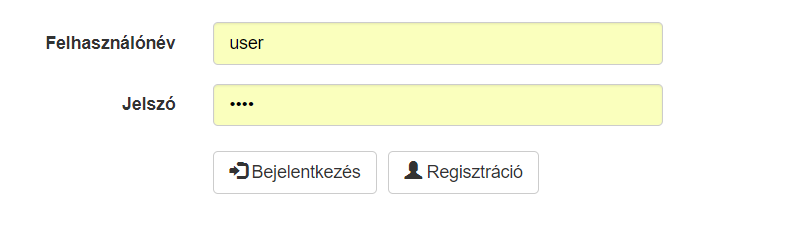
\includegraphics[scale=0.8]{kepek/login.png}
\caption{Bejelentkező felület}
\label{fig:architecture}
\end{figure}

\section{Egyszerű user funkciói}

A továbbiakban az alapfunkciókat a szerint fogom leírni, hogy melyik felhasználói csoport számára érhetők el. A vásárlók által elérhető szolgáltatásokkal kezdem

\subsection{Éttermek listázása}

A vásárlók számára adott egy olyan funkció, hogy ki tudják listázni az adatbázisban szereplő összes éttermet. Az éttermek egymás alatt, egy táblázatban jelennek meg. A táblázatban szerepel az étterem logója, neve, rövid leírása, címe, a várható kiszállítási idő, kiszállítási költség, a minimális rendelés összege és egy gomb, amire kattintva az oldal tovább irányítja a vásárlót az adott étterem étlapjához (\ref{fig:restaurants}. ábra).

A vásárlónak lehetősége van szűrni az éttermeket város szerint, ami segíti őket abban, hogy csak a számukra elérhető távolságban levő éttermek kínálatát lássák.

\begin{figure}
\centering
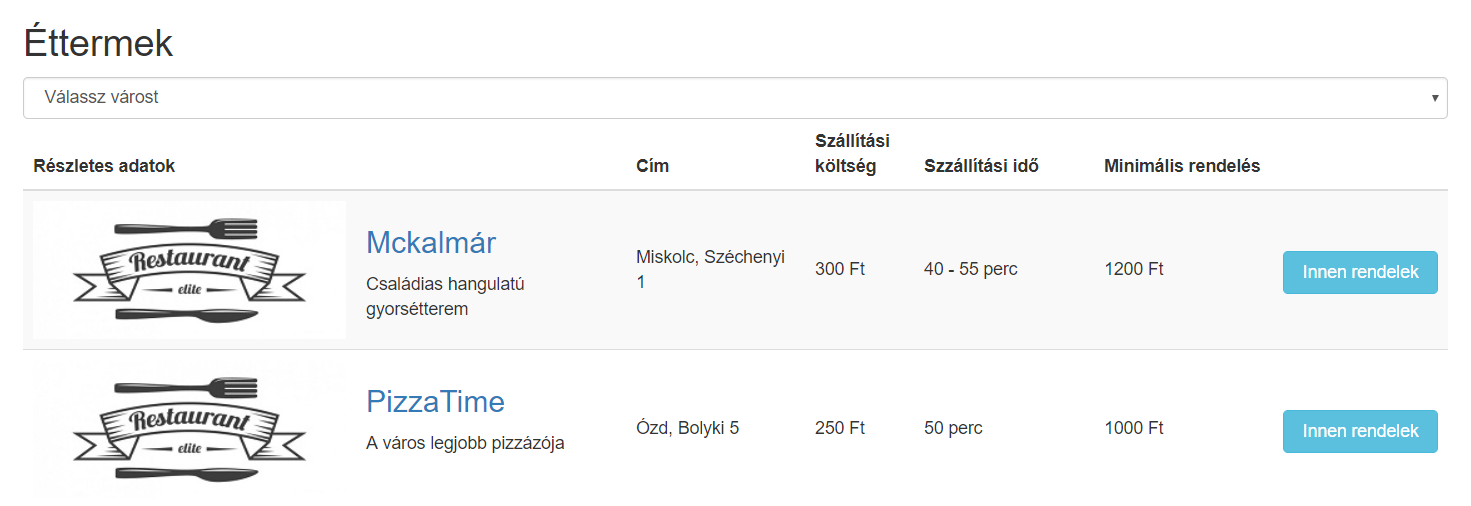
\includegraphics[scale=0.5]{kepek/restaurants.png}
\caption{Az éttermek listázása}
\label{fig:restaurants}
\end{figure}

\subsection{Étlap}

Miután a vásárló kiválasztotta a neki legszimpatikusabb éttermet, az „innen rendelek” gombra kattintva el lehet érni az adott étterem étlapját.

Az ételek egymás alatt, egy táblázatban jelennek meg (\ref{fig:menu}. ábra). A táblázat egyes soraiban egy-egy étel szerepel, az oszlopaiban pedig az adott étel adatai, többek között neve, egy kép róla, az ára és egy rövid leírás róla. A táblázat jobb szélső oszlopában egy „kosárba” feliratú gomb található, amit megnyomva a kiválasztott termék belekerül a felhasználó kosarába.

Az étlap felett van egy legördülő menü, ahol vásárló kiválaszthatja, hogy milyen típusú ételek között szeretne válogatni, milyen típusút szeretne rendelni. Az étel típus kiválasztása után, az ételek listája szűrve lesz az adott típus szerint, tehát csak a kívánt típusú ételek fognak megjelenni a táblázatban.

Miután a vásárló kiválasztotta a rendelni kívánt termékeket, és hozzáadta őket a kosárhoz, megjelenik a felületen a „fizetés” gomb, amire kattintva elérjük a fizetés funkciót.

\begin{figure}
\centering
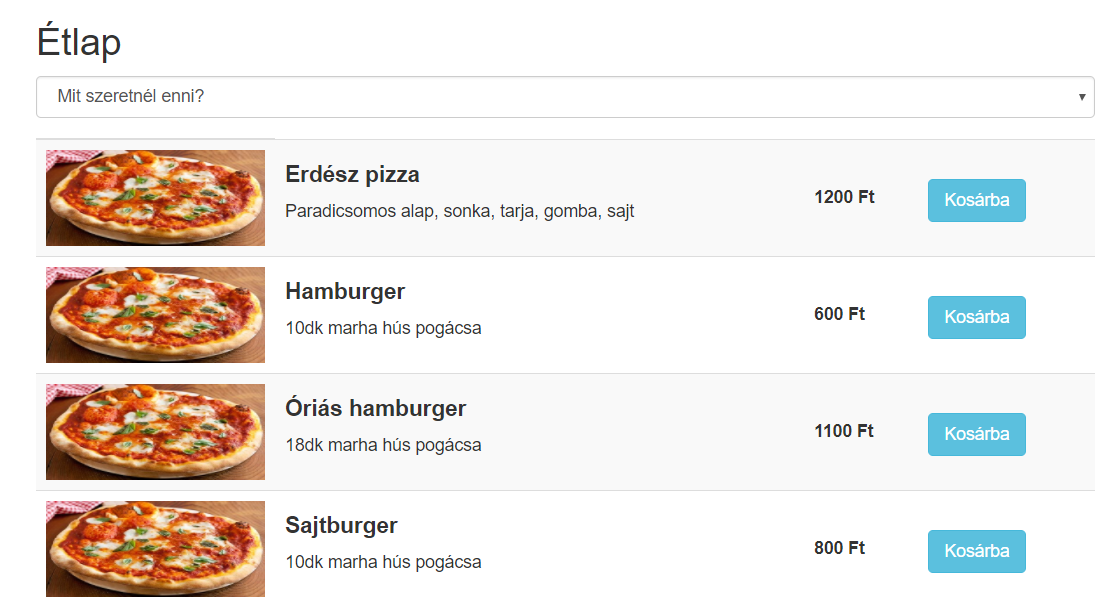
\includegraphics[scale=0.5]{kepek/menu.png}
\caption{Kép egy, az alkalmazásban megjelenített étlapról}
\label{fig:menu}
\end{figure}

\subsection{Fizetés}

A felhasználói felületen a kosár az étlap mellett, jobb oldalon található szintén egy táblázatos megoldással. A hozzáadott termékek neve és ára egymás alatt jelenik meg, egy végösszeggel a táblázat alján (\ref{fig:order}. ábra).

A kosár legalsó sorában egy „fizetés” gomb található. A gombra kattintva felugrik egy modal ablak, ahol egy legördülő menüből lehet kiválasztani a kívánt fizetési módot. Az alkalmazásban korlátozott számú fizetési lehetőség van, ami éttermenként változó lehet. Hogy egy étterem milyen fizetési lehetőségeket biztosít, azt az adott étterem felvitelekor kell megadni.

\begin{figure}
\centering
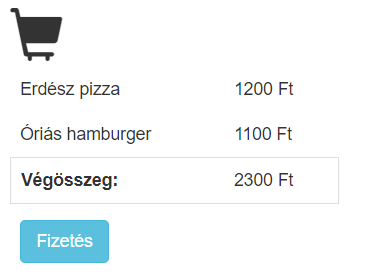
\includegraphics[scale=0.8]{kepek/order.png}
\caption{A vásárlás tételei összeggel és végösszeggel megjelenítve}
\label{fig:order}
\end{figure}

A kívánt fizetési lehetőség kiválasztása után (\ref{fig:payment}. ábra) a fizetés gombbal lehet véglegesíteni a megrendelést. Ilyenkor kapunk értesítést, hogy sikeres volt a rendelés.

\begin{figure}
\centering
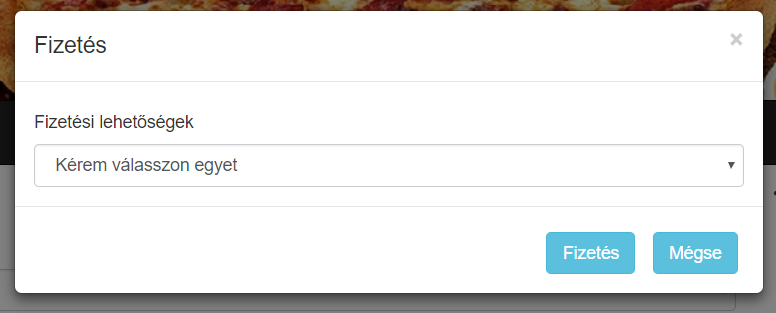
\includegraphics[scale=0.8]{kepek/payment.png}
\caption{A fizetési mód kiválasztása}
\label{fig:payment}
\end{figure}

\subsection{Profilom}

A profilom funkció kilistázza a bejelentkezett felhasználó adatait. Egy táblázatba foglalva kilistázza a felhasználó teljes nevét, felhasználónevét, email címét, telefonszámát, jutalompontját és címét/címeit. Egy felhasználónak akár több különböző szállítása címe is. A táblázat legalsó sorában van egy gomb „jelszó módosítása” felirattal (\ref{fig:profile}. ábra).

Jutalompontot a rendelések után kap a vásárló, minden elköltött 100 forint után egy jutalom pontot ír jóvá a rendszer. Az összegyűjtött pontokat, fizetéskor be lehet váltani, ilyenkor a beváltott pontok összege levonásra kerül a rendelés végösszegéből.

\begin{figure}
\centering
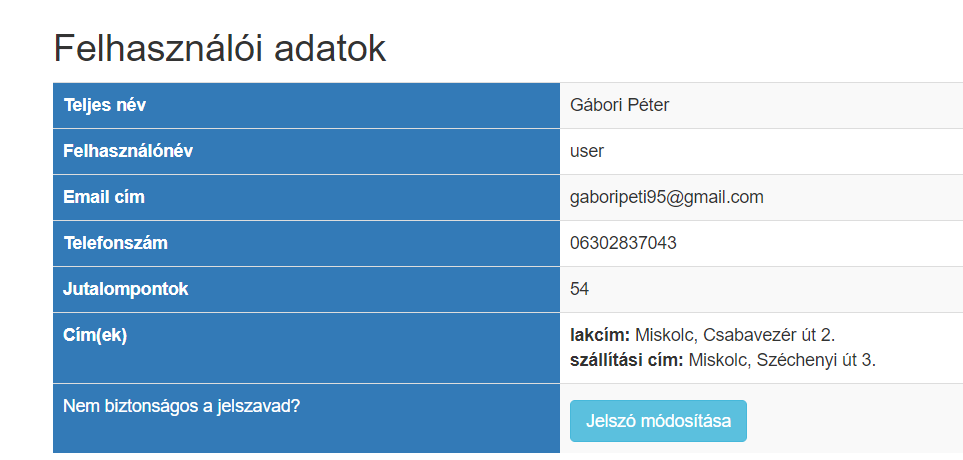
\includegraphics[scale=0.6]{kepek/profile.png}
\caption{Felhasználói adatok megjelenítése}
\label{fig:profile}
\end{figure}

A „Jelszó módosítása” gombra kattintva megjelenik egy űrlap, ahol a felhasználónak lehetősége van megváltoztatni a jelenlegi jelszavát (\ref{fig:password}. ábra). Meg kell adnia a jelenlegi jelszavát, majd az új jelszavát és végül meg kell erősítenie az új jelszót. Ha kitöltötte a bemeneti mezőket, a „Mentés” gombra kattintva megtörténik a jelszó cserélő funkció meghívása. Amennyibben a jelenlegi jelszó helyes, az új jelszó megfelel a kritériumoknak és megegyezik a megerősített jelszóval, megtörténik a jelszó módosítása.

\begin{figure}
\centering
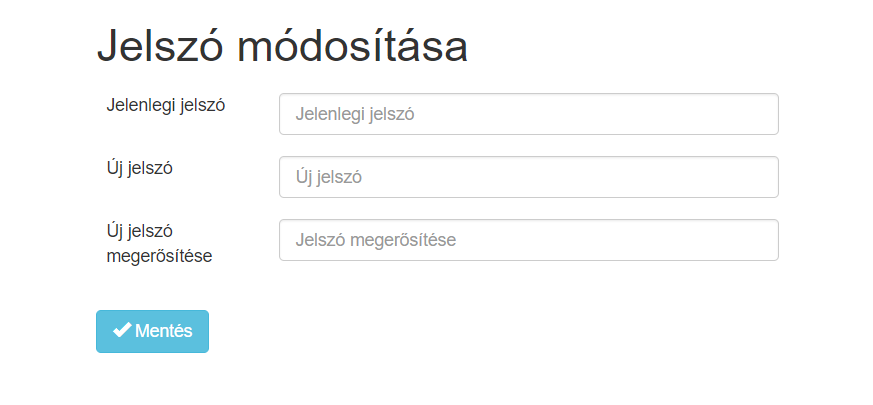
\includegraphics[scale=0.8]{kepek/password.png}
\caption{Jelszó megváltoztatása}
\label{fig:password}
\end{figure}

\section{Étterem tulajdonos funkciók}

\subsection{Éttermeim}

Az éttermeim funkció kilistázza a felhasználó adatbázisban szereplő éttermeit. Az éttermek táblázatos elrendezésben jelennek meg a felületen, a táblázat minden egyes sora, egy éttermet reprezentál. A táblázat oszlopaiban az éttermek különböző adatai találhatók, többek között az étterem logója, neve címe. A jobb szélső oszlopban három gomb található, „Étlap szerkesztése”, „Étterem szerkesztése” és a „Rendelések” (\ref{fig:my_restaurants}. ábra).

\begin{figure}
\centering
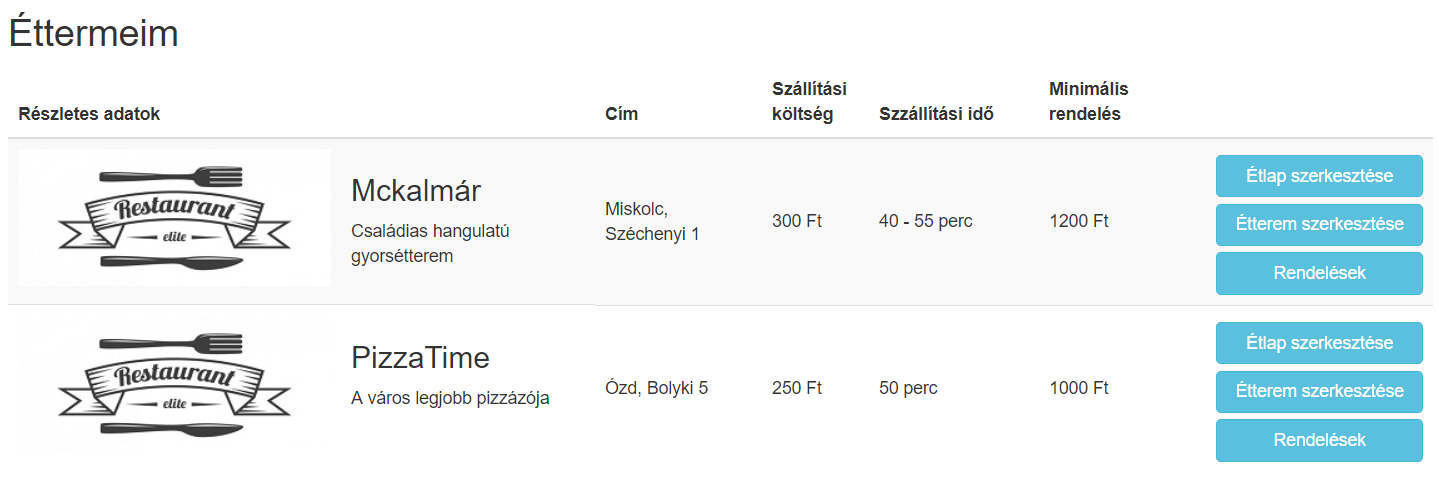
\includegraphics[scale=0.5]{kepek/my_restaurants.png}
\caption{A saját éttermek kilistázása}
\label{fig:my_restaurants}
\end{figure}

\subsection{Étlap szerkesztése}

Az étlap szerkesztése menüpont kiválasztása utána, egy táblázatot fogunk látni az adott étterem által forgalmazott ételekről és ezen ételek adatairól. Az elrendezés hasonló a user oldalon látott étlapok elrendezéséhez.

Az ételek egymás alatt, egy táblázatban jelennek meg. A táblázat egyes soraiban egy-egy étel szerepel, az oszlopaiban pedig az adott étel adatai. A táblázat jobb szélső oszlopában két gomb található, „Étel szerkesztése”, „Étel törlése”. A táblázat alatt egy „Étel felvitele” feliratú gomb van.

A táblázat felett egy legördülő menü van, amelynek segítségével a tulajdonos rá tud szűrni a különböző ételtípusokra, ezáltal könnyebben megtalálhatja a szerkeszteni, vagy törölni kívánt terméket. Az étel típus kiválasztása után, az ételek listája szűrve lesz az adott típus szerint, tehát csak a kívánt típusú ételek fognak megjelenni a táblázatban (\ref{fig:new_meal}. ábra).

\begin{figure}
\centering
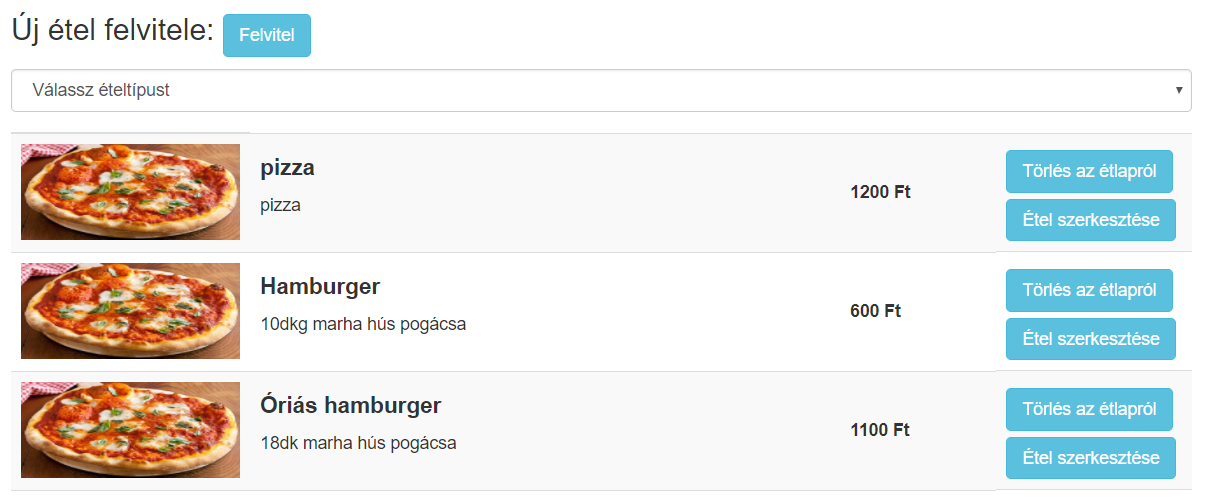
\includegraphics[scale=0.5]{kepek/new_meal.png}
\caption{Új étel hozzáadása}
\label{fig:new_meal}
\end{figure}

\subsection{Étel törlése}

Az étterem tulajdonosnak lehetősége van testre szabnia az étterme által biztosított kínáltaot. Vannak bizonyos ételek, melyeket csak szezonálisan lehet elkészíteni az alapszükségletük miatt, vagy csak valamilyen oknál fogva úgy dönt a vezetőség, hogy le kell kerülnie az étlapról. Ilyenkor van szükség az étel törlés funkcióra. Az „Étel törlése” gombra kattintva meghívásra kerül az étel törlése funkció, melynek hatására a kiválasztott étel törlődik a megjelenített ételek listájából, és törlődik az adatbázisból is.

\subsection{Étel szerkesztése}

Az étel szerkesztése funkcióval lehetőséget biztosítok az étterem tulajdonos számára, az étlapon szereplő termékek adatainak módosítására. Tehát ha egy adott ételnek megváltozik az ára vagy például az összetétele, akkor nem kell törölni azt, majd az új adatokkal ismét felvinni az adatbázisba. Mindössze rá kell kattintani a szerkeszteni kívánt termék sorában található gombok közül az „Étel szerkesztése” gombra, melynek hatására meghívódik az étel szerkesztése funkció.

Egy űrlapot fogunk látni, ahol a szükséges módosítások elvégzése után, a mentés gombbal lehet véglegesíteni a módosítást (\ref{fig:edit_meal}. ábra).

\begin{figure}
\centering
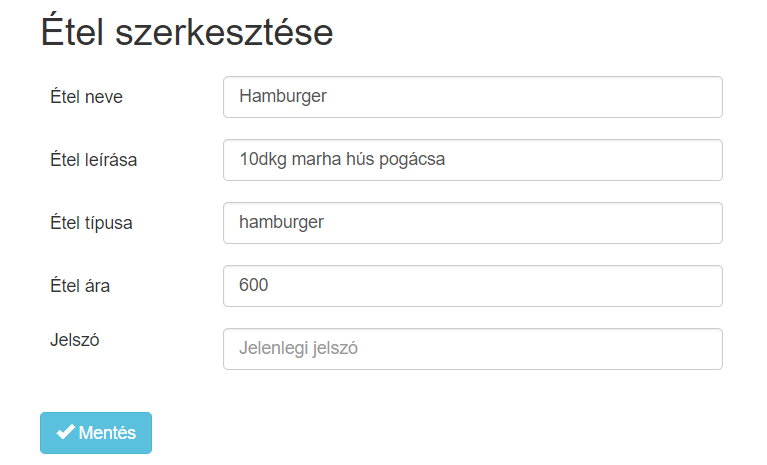
\includegraphics[scale=0.8]{kepek/edit_meal.png}
\caption{Egy étel adatainak szerkesztése}
\label{fig:edit_meal}
\end{figure}

\subsection{Étel felvitele}

Az étel felvitel gombra kattintva egy űrlap fog betöltődni. Az űrlap beviteli mezőkből áll, melyekkel az étlapra felvinni kívánt étel adatait tudjuk elküldeni a szervernek. Meg kell adni többek között az étel nevét, árát és típusát. Amennyiben minden szükséges mezőt kitöltöttünk a „Felvitel” gombra kattintva lehet véglegesíteni a műveletet.

\begin{figure}
\centering
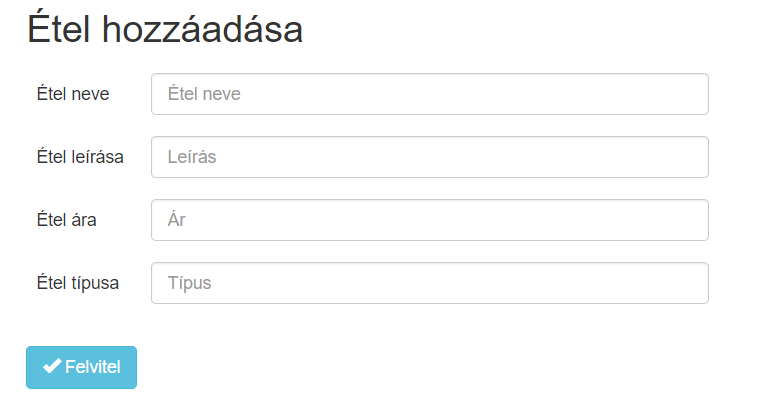
\includegraphics[scale=0.8]{kepek/add_meal.png}
\caption{Új étel felvitele az étlapra}
\label{fig:add_meal}
\end{figure}

\subsection{Rendelések}

Ahogy már említettem, az éttermeim funkció kilistázza a felhasználó adatbázisban szereplő éttermeit. Ilyenkor az éttermek táblázatos formában jelennek meg, minden étterem sorában szerepel egy „Rendelések” feliratú gomb. Erre a gombra kattintva a szerver kilistázza az adott étteremhez tartozó megrendeléseket, tehát azokat a rendeléseket, amiket ebben az étteremben adtak le a vásárlók. A rendelések táblázatos formában jelennek meg a felületen, egy sor egy rendelés. A táblázat oszlopaiban az egyes rendeléshez tartozó rendelési adatok vannak megjelenítve. Az adatok között szerepel a rendelő neve, rendelés időpontja, a megrendelt termékek, a rendelés összege és a fizetési módja.

\subsection{Étterem szerkesztése}

Egy étteremtulajdonosnak lehetősége lesz az éttermei adatainak módosítására. A szerkesztendő étterem sorában rá kell klikkelni az étterem szerkesztése gombra. Kattintás után megjelenik egy űrlap, amire fel kell vinni a módosítandó adatokat. Az adatok megadását követően a mentés gombbal lehet véglegesíteni a módosításokat (\ref{fig:edit_meal}. ábra).

\begin{figure}
\centering
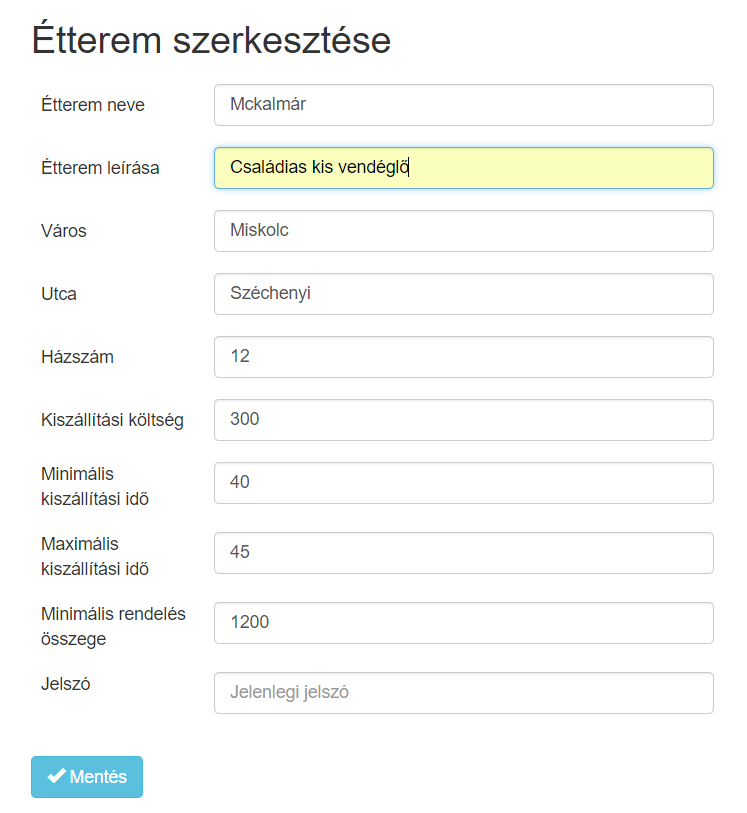
\includegraphics[scale=0.8]{kepek/edit_restaurant.png}
\caption{Étterem adatainak szerkesztése}
\label{fig:edit_restaurnt}
\end{figure}

\subsection{Étterem hozzáadása}

Egy étterem tulajdonosnak több étterme is lehet az adatbázisban. Az étterem hozzáadása menüpont alatt van lehetőség egy újabb éttermet felvinni. 
A menüpontra kattintva egy űrlapot fogunk látni, ahol a beviteli mezők egymás alatt helyezkednek el. Az egyes beviteli mezőkben az étterem különböző adatait lehet megadni. Az étterem nevét, leírását, címét. Ha elkészültünk az adatok megadásával, a „Felvitel” gombbal lehet véglegesíteni ezt a műveletet (\ref{fig:add_restaurant}. ábra).

\subsection{Profilom}

A profilom funkció az étterem tulajdonosok szempontjából is ugyanaz, mint a vásárlóknál. Kilistázza a bejelentkezett felhasználó adatait. Egy táblázatba foglalva kilistázza a felhasználó teljes nevét, felhasználónevét, email címét, telefonszámát és címét. A táblázat legalsó sorában van egy gomb „jelszó módosítása” felirattal.

A jelszó módosítás is ugyanúgy működik, mint a vásárlóknál. A „Jelszó módosítása” gombra kattintva megjelenik egy űrlap. Meg kell adni a jelenlegi jelszót, majd az új jelszót és végül meg kell erősíteni az új jelszót. A „Mentés” gombra kattintva megtörténik a jelszó cserélő funkció meghívása. Amennyibben a jelenlegi jelszó helyes, az új jelszó megfelel a kritériumoknak és megegyezik a megerősített jelszóval, megtörténik a jelszó módosítása.

\section{Éttermi nyilvántartás}

Az éttermi nyilvántartás egy roppantul összetett problémakör. Az ilyen szoftverek tervezésénél figyelembe kell venni, hogy nincs két egyforma vendéglátó egység, tehát a szoftvert mindig az adott vállalkozáshoz kell igazítani. Nyilván kell tartani a rendeléseket, a raktárkészletet, a felhasználókat, törzsvendégek kezelését. A szoftverrel szemben elvárás, hogy megkönnyítse a szoftverrel dolgozók munkáját, átláthatóvá tegye az üzletvezetők számára az üzlet menetét és az ellenőrzést. Szintén elvárás, hogy könnyen kezelhető és rugalmasan bővíthető legyen.

\subsection{Rendelésnyilvántartás}

Rendelések esetén számos adatot nyilván kell tartani. Fontos, hogy ki rendelt, mikor, melyik étteremből, mit, mennyit és mivel fizetett. Menedzselni kell futárszolgálatot, betartani a kiszállítási időt. Biztosítani kell a vásárlók számára pontos leírást az ételekről, választási lehetőséget a fizetési lehetőségek között, estleg vegyes fizetési lehetőségeket egy számlán belül.

\subsection{Készletnyilvántartás}

Vannak éttermi nyilvántartó szoftverek, melyek lehetőséget biztosítanak teljes körű raktárkészlet kezelésre, egy vagy akár több raktárral is. Ebbe beletartozik az alapanyagok bevételezése, selejtezés, abban az esetben, ha több raktár is van, akkor raktárok közötti átvételezés.
Ebbe a problémakörbe tartozhat még a menü összeállítása, előrendelések kezelése, a termékekhez tartozó receptúrák kezelése, tehát nyilvántartása és módosítása.

\subsection{Törzsvendégek kezelése}

A vásárlók teljeskörű nyilvántartása az ilyen típusú szoftverek esetén alap elvárás. A rendszeresen vásárló felhasználók számára nyújtani kell valamilyen fajta plusz szolgáltatást, amivel meg lehet hálálni a hűségüket, és el lehet azt érni, hogy továbbra is ezt a szoftvert használják. Erre a problémára nyújtanak megoldást a különböző törzsvásárlói kedvezmények.

\subsection{Ellenőrzés}

Egy sikeres vállalkozáshoz szükség van a folyamatos ellenőrzésre, az üzletvezetőnek mindig át kell látnia az üzlet menetét. Az ilyen típusú nyilvántartó rendszerek egy része lehetőséget biztosít a termékek szerinti fogyások kimutatására, ez egy nagyon fontos statisztika, amely megmutatja, hogy egy adott időszakban melyik termék volt a legnépszerűbb, tehát fogyott belőle a legtöbb, illetve, hogy melyikből fogyott a legkevesebb. Biztosítják az alapanyagok készletszintjének figyelését.

Fontos statisztikákat, grafikonokat állítanak elő egy adott időszakra, melyek nélkülözhetetlenek a további üzleti lépések meghozatalához, a sikeres üzleti élethez. Kimutatások a pillanatnyi alapanyag készletről, ezeknek lekérdezése, a lekérdezések és kimutatások exportálása.

\subsection{Elterjedt megoldások}

Az internetet böngészve számos étterem nyilvántartó szoftvert lehet találni. Vannak köztük online webalkalmazások, és letölthető desktop alkalmazások is. Összeszedtem a már létező alternatívák közül a Magyarországon legelterjedtebbeket, és egy táblázatban néhány szempont alapján összehasonlítottam őket (\ref{tab:features}. táblázat).

\begin{table}
\centering
\begin{tabular}{|l|c|c|c|c|c|}
\hline
Program neve & felhasználókezelés & profil & könyvelés & feladatkezelés & készletnyilvántartás \\
\hline
eSystem & van & általános webshop & van & igen & igen \\
\hline
R-keeper & nincs & teljesen egyedi & nincs & igen & igen \\
\hline
MultiStore & nincs & teljesen egyedi & van & igen & igen \\
\hline
Stand-Mágus & van & teljesen egyedi & van & igen & igen \\
\hline
\end{tabular}
\caption{Elterjedt funkciók}
\label{tab:features}
\end{table}

A táblázat első oszlopában a szoftver neve szerepel. A második oszlopban a felhasználókezelés, ami azt takarja, hogy a szoftver funkció között van e vendég nyilvántartás, tehát, hogy lehet e regisztrálni a vendégeket. A harmadik oszlopban a szoftver profilját, arculatát jellemeztem. A negyedik oszlopban azt vizsgáltam, hogy van e integrált könyvelés funkció az alkalmazásban. Az 5. oszlopban feladatkezelés alatt azt értettem, hogy a pénztárgép funkcióit is a szoftver látja e el. A hatodik azaz utolsó oszlopban a szoftver raktár készlet kezelését vizsgáltam.

Az én alkalmazásom a vásárlók teljes körű nyilvántartására, rendelések nyilvántartására és az ezekből alkotott kimutatásokra, statisztikákra fog összpontosulni. Az alkalmazásom célja, a házhoz szállítást nyújtó éttermek összegyűjtése, az üzletvezetők feladatának, éttermek menedzselésének megkönnyítése, és a rendelők számára a minél egyszerűbb ételrendelés biztosítása. Az hasonló célú és felépítésű szoftvereket online ételrendelési portálnak szokták nevezni.

A magyar piacon jelenleg három online ételrendelési portál óriás van, a NetPincér, a Pizza.hu és a Falatozz.hu. Ezek a portálok közvetítő szerepet játszanak a megrendelő és a kiszállítást lebonyolító étterem között. Az éttermeknek ez egy nagyon jó marketing fogás, segít nekik az ügyfélkör kibővítésében, a megrendelőknek, meg leegyszerűsítik az online ételrendelést, azzal, hogy egy oldalon megtalálják a környéken lévő összes vendéglátó egység kínálatát.

Az alkalmazásom abban különbözik ezektől az online étrendelési portáloktól, hogy míg ezek a portálok úgymond csak közvetítő szerepet vállalnak, nem feltétlenül tartják nyilván az adatokat, a partner cégek egyébként is rendelkeznek egy saját étterem nyilvántartói rendszerrel és általában webes rendelő felülettel is. Addig az általam készített alkalmazás biztosítja a rendelésnyilvántartást, a vásárlónyilvántartást és a szerzett adatokból olyan statisztikákat, kimutatásokat állít elő, melyek elengedhetetlenek egy sikeres vállalkozáshoz.
